\chapter{Influence Diagrams \& Utility Nodes}
\label{ch-influ-diag}

This chapter is based on Refs.\cite{sha-influ-diag}, \cite{limid-one} and \cite{cabanas2017}.

An {\bf Influence Diagram (ID)} is
a DAG that generalizes a bnet by adding
2 new types of nodes. IDs have 3 types of nodes: chance, decision and utility (a.k.a value) nodes, represented, respectively, by ovals, rectangles and diamonds.\footnote{Since our
bnet drawing software {\tt xypic} cannot draw diamond frames for nodes,
in this book, we sometimes 
represent chance, decision
and utility nodes by no-frames, rectangles and doubly-lined rectangles, respectively.}

Fig.\ref{fig-simple-id} and the information printed in blue 
that follows it, are a simple example of an ID.
\begin{figure}[h!]
$$
\xymatrix{
*++[F]{\rvd_1}\ar[r]\ar[rd]\ar[d]
&\rvb\ar[d]
&\rvc\ar[l]\ar[d]
\\
*++[F=]{\rvu_1}
&*++[F]{\rvd_2}\ar[r]
&*++[F=]{\rvu_2}
}
$$
\caption{Simple example of an Influence Diagram.
Chance, decision and utility nodes
are indicated by a no-frame, rectangle and doubly-lined
rectangle, respectively.}
\label{fig-simple-id}
\end{figure}

\begin{itemize}
\item Chance Nodes:
\beq\color{blue}
P(b|c, d_1=0)=\left[\begin{array}{cc}
.1&.3
\\
.9&.7
\end{array}
\right]_{b,c, d_1=0}
,\;\;
P(b|c, d_1=1)=\left[\begin{array}{cc}
.2&.4
\\
.8&.6
\end{array}
\right]_{b,c, d_1=1}
,\;\;
P(c)=\left[\begin{array}{c}
.6
\\
.4
\end{array}
\right]_{c}
\eeq
\item Utility nodes:
\beq\color{blue}
u_1(d_1)=
\left[
\begin{array}{c}
10
\\
-23
\end{array}
\right]_{d_1}
,\;\;
u_2(d_2, c)=
\left[
\begin{array}{cc}
2&-8
\\
45&7
\end{array}\right]_{d_2, c}
\eeq
\item Decision nodes:

{\color{blue}$P(d_1)$ and $P(d_2|b, d_1)$ 
are deterministic TPMs obtain by
optimization. They maximize $u=u_1+u_2$.}
\end{itemize}




 Table \ref{tab-id-nodes} compares these 3 types of nodes in an  ID. Note that a decision node
 is a deterministic node\footnote{Deterministic nodes
 are defined by Eq.(\ref{eq-def-det-node})}, but its TPM is 
 not known a priori. Instead, it is derived by an optimization algorithm which maximizes the total utility.

% Please add the following required packages to your document preamble:
% \usepackage[table,xcdraw]{xcolor}
% Beamer presentation requires \usepackage{colortbl} instead of \usepackage[table,xcdraw]{xcolor}
\begin{table}[h!]
\begin{tabular}{|l|l|l|l|}
\hline
                                                                                            & \cellcolor[HTML]{FFFFC7}\begin{tabular}[c]{@{}l@{}}Chance node \\ (oval)\end{tabular} & \cellcolor[HTML]{FFFFC7}\begin{tabular}[c]{@{}l@{}}Decision node\\ (rectangle)\end{tabular} & \cellcolor[HTML]{FFFFC7}\begin{tabular}[c]{@{}l@{}}Utility node\\ (diamond)\end{tabular} \\ \hline
\cellcolor[HTML]{FFFFC7}type of states                                                      & discrete                                                                     & discrete                                                                      & continuous                                                                             \\ \hline
\cellcolor[HTML]{FFFFC7} deterministic?                                                   & Not in general                                                                        & Yes                                                                                      & Yes                                                                                    \\ \hline
\cellcolor[HTML]{FFFFC7}transition info\footnote{by \qt{transition info}
of a node, we
mean \qt{personal} node info
other than a list of the states of the node and a list 
of its parent nodes}                                                    & TPM                                                                                   & 
deterministic TPM                                                                                  & \begin{tabular}[c]{@{}l@{}}utility function,\\ not normalized
\end{tabular}
\\ \hline
\cellcolor[HTML]{FFFFC7}\begin{tabular}[c]{@{}l@{}}
transition info \\ known a priori\end{tabular} & Yes                                                                                   & 
No                                                      & Yes                                                                           \\ \hline
\cellcolor[HTML]{FFFFC7}children type                                                       & chance, decision, value                                                               & chance, decision, value                                                                  & None                                                                                                                                                                   \\ \hline
\end{tabular}
\caption{Comparison of the 3 types
of nodes in an influence diagram.}
\label{tab-id-nodes}
\end{table}

\section{Definitions}
Let

$\rvc.=$ set of {\bf chance nodes}

$\rvd.=$ set of {\bf decision nodes}.
Assume $\rvd_i$ are in chronological (a.k.a., topological)
order, i.e., $\rvd_i$ occurs before 
(or concurrent with)  $\rvd_{i+1}$ for all $i$.

$\rvu.=$ set of {\bf utility nodes}. Often, utility nodes are called {\bf value nodes} and only their sum is called a utility node.

$\rvX.= \rvc. \cup \rvd. \cup \rvu.$ all nodes

$pa(\rvX_i)=$ parents of node $\rvX_i$

$va(\rvX_i)=$ set of values (a.k.a.) states that 
node $\rvX_i$ can assume.


$\rve.=$ {\bf evidence nodes}, the subset $\rve.$  of the chance nodes $\rvc.$ that is {\bf apriori observed}
(i.e. measured before the experiment starts). If a decision node has a 
chance node as a parent,
we will assume it is measured immediately before the decision is made,
not apriori.


$u_i(pa(\rvu_i))=$ {\bf partial utility function}

$u(\rvc., d.)=\sum_i u_i(pa(\rvu_i))$ {\bf total utility function }


\begin{itemize}

\item {\bf Chance node partition}

Given $nd$ decision nodes $\{\rvd_i\}_{i=1}^{nd}$, we partition the set of chance nodes $\rvc.$
into $nd+1$ disjoint subsets $\{\rv{\calc}_i\}_{i=0}^{nd}$ 
 in such a way that
all nodes in $\rv{\calc}_{i-1}$ occur before (or concurrent with) $\rvd_i$, and
$\rvd_i$  occurs before (or concurrent with) all nodes in $\rv{\calc}_{i}$.
Thus,

\beq
\rv{\calc}_0\prec \rvd_1  \prec 
\rv{\calc}_1\prec \rvd_2
\ldots\prec \rv{\calc}_{nd-1}\prec \rvd_{nd}
\prec \rv{\calc}_{nd}
\eeq
where $\prec$ is the partial chronological (a.k.a., topological)
ordering.



\item{\bf Optimal Strategy (or Policy)}

Define the conditional probabilities
\beq
P(d_i|pa(d_i))=
\delta(d_i, \Delta_i(pa(d_i)))
\eeq
and

\beq
P(c.|d.)=\prod_{i}P(c_i|pa(c_i))
\eeq
If $\rvc_i$ is evidence,
replace $P(c_i|pa(c_i))$
by $\delta(c_i, c_i^*)$.


Let
\beq
\underbrace{\rv{\calc}_0}_{\cald_0},
\underbrace{ \rvd_1,\rv{\calc}_1 }_{\rv{\cald}_1}, 
\underbrace{\rvd_2, \rv{\calc}_2}_{\rv{\cald}_2}, 
\ldots, 
\underbrace{\rv{\cald}_{nd},\rv{\calc}_{nd}}_{ \cald_{nd}}
\eeq
and $\cald_{<i}= \cup_{j=1}^{i-1}\cald_j$.

For $i=1, 2, \ldots ,nd$, let

\beq
\max_{\cald_i}=
\max_{d_i}\sum_{\calc_{i}}
\eeq
\beq
\argmax_{\cald_i}=
\argmax_{d_i}\sum_{\calc_{i}}
\eeq

\beq
\Psi_{i}^*( \cald_{<i})=
\max_{\cald_i}\underbrace{\max_{\cald_{i+1}}
\ldots \max_{\cald_{nd}}
P(c.|d.)u(c., d.)}_{\Psi_{i+1}^*(\cald_{<i+1})}
\eeq

\beq
\Delta_{i}^*(\cald_{<i})=
\argmax_{\cald_i}\underbrace{\max_{\cald_{i+1}}
\ldots \max_{\cald_{nd}}
P(c.|d.)u(c., d.)}_{\Psi_{i+1}^*(\cald_{<i+1})}
\eeq


The {\bf optimum policy} is defined by

\beq
\Delta^*. = (\Delta_1^*, \Delta_2^*, \ldots,
\Delta_{nd}^*)
\eeq
and the {\bf Maximum Expected Utility} (MEU) by
\beq
MEU =\sum_{\calc_0}\Psi_1(\calc_0)
\eeq

Thus, for example, if $nd=3$, we have 3 max-expectation problems to be performed 
in the following order:

\beq
\left\{
\begin{array}{ll}
1)&\Psi_3(\cald_{<3} )=P(c.|d.)u(c., d.)
\\
2)&\Psi_{2}(\cald_{<2}) = \max_{\cald_2}\Psi_{3}(\cald_{<3})
\\
3)&\Psi_{1}(\calc_0)=\Psi_{1}(\cald_{<1}) = \max_{\cald_1}\Psi_{2}(\cald_{<2})
\\
4) &MEU = \sum_{\calc_0}\Psi_{1}(\calc_0)
\end{array}
\right.
\eeq
Note that $\Psi_i()$ at time  $i$
depends solely on the decisions $\cald_{<i}$
in its past.

\begin{mdframed}[hidealllines=true,backgroundcolor=blue!10]
On first encountering this algorithm, the
reader might question how to do the maximization
over $d_i$
without knowing $\cald_{<i}$. It turns out that due to d-separation, all you have to do is pick one instatiation 
and stick with it throughout when needed. The result for the 
optimum policy and MEU 
will
be independent of the instantiation you chose.
This is clear if you think of 
$
\rv{\cald}_0\rarrow \rv{\cald}_1\rarrow\cdots\rarrow 
 \rv{\cald}_{nd}
$
as a Markov chain. When you maximize over $d_i$
you hold it fixed, and $P(\calc_i|d_i, \cald_{<i}) =
P(\calc_i|d_i)$.

\end{mdframed} 



\item {\bf Limited Memory ID (LIMID)}. 

LIMIDs were first introduced 
in Ref.\cite{limid-one}. According to that reference, LIMIDs are
\qt{multistage
decision problems in which the traditional assumption of no forgetting is
relaxed.}
Note that \qt{multistage decision problems} is another term
for a dynamic bnet (see Chapter \ref{ch-dyn-bnets}).

Here is an example of LIMIDs.
Figs.\ref{fig-pre-limid} and \ref{fig-post-limid}
come from Ref.\cite{limid-one} and describe pig farming
at various times $T=\{1,2,3,4\}$.

Node $\rvh_i\in\bool$
refers to the health of a pig at time $i$.

Node $\rvt_i\in \bool$ refers to a test 
conducted on the pig at time $i$.

Node $\rvd_i\in \bool$ refers to a decision 
made by the farmer at time $i$ on whether to medicate the pig.

Node $\rvu_i\in \RR$ refers to the utility (monetary value)  
of medicating the pig at time $i$.

 
Fig.\ref{fig-pre-limid} shows a dynamic bnet that
obeys the {\bf no forgetting} assumption so every decision is
privy to the state of all previous decision and some chance nodes.
Fig.\ref{fig-post-limid} shows the same bnet as 
Fig.\ref{fig-pre-limid} after all arrows entering a decision $\rvd_i$ and originating at an earlier time, have been removed.



\begin{figure}[h!]
\centering
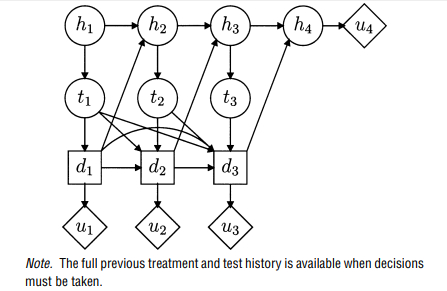
\includegraphics[width=4in]
{influ-diag/pre-limid.jpg}
\caption{Pig farming ID that obeys the \qt{no-forgetting}
assumption.  
}
\label{fig-pre-limid}
\end{figure}


\begin{figure}[h!]
\centering
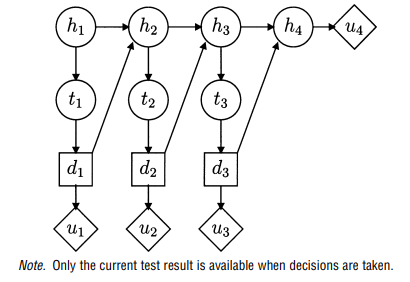
\includegraphics[width=4in]
{influ-diag/post-limid.jpg}
\caption{Pig farming ID that obeys the  LIMID
assumption. This ID is the same as the ID of Fig.\ref{fig-pre-limid},
except that the arrows pointing to a decision and originating at a previous time, have been removed.}
\label{fig-post-limid}
\end{figure}

\item {\bf Finding optimal strategy }


Ref.\cite{sha-influ-diag} proposes the following 3 exact methods for
finding the optimal strategy of an ID.
\begin{enumerate}
\item conversion to a decision
tree 
\item calculation directly from ID, using Variable
Elimination Algorithm (VEA)
\item conversion to a rooted cluster tree.
\end{enumerate}

All 3 methods require  reversing some arrows. To reverse
an arrow, $\rvx\rarrow \rvy$, we add dummy arrows going into $\rvx$ or into
$\rvy$ so that $pa(\rvx)=pa(\rvy)= \calc$. After that, we use Bayes rule conditioned on $\calc$.


\beq
P(x|y, \calc) = \frac{P(y|x, \calc)P(x|\calc)}{\sum_x \text{ numerator}}
\eeq




In the next section,
we discuss method 2 (VEA).

\end{itemize}

\section{Variable Elimination Algorithm (VEA)}


VEA utilizes the following operations:
\begin{enumerate}
\item Summing over barren (i.e., childless) chance nodes.
\item Reversing $\rvx\rarrow \rvy$
to $\rvy\rarrow \rvx$
using Bayes Rule.
\beq
\xymatrix{
\corchete{a.}\ar[d]
&\corchete{b.}\ar[dl]\ar[dr]
&\corchete{c.}\ar[d]
\\
x\ar[rr]&&y
}
\xymatrix{\\\text{\;\;equals\;\;}}
\xymatrix{
\corchete{a.}\ar[d]\ar[drr]
&\corchete{b.}\ar[dl]\ar[dr]
&\corchete{c.}\ar[d]\ar[dll]
\\
x&&y\ar[ll]
}
\eeq

\item Summing over the states of a chance node. Suppose
$\rvx\rarrow \rvu$ 
where $\rvx$ is a chance node and $\rvu$
is a utility node, and $\rvx$ has only one child $\rvu$. Then
\beq
\xymatrix{
\corchete{a.}\ar[d]
&\corchete{b.}\ar[dl]\ar[dr]
&\corchete{c.}\ar[d]
\\
x\ar[rr]
&&\diamante{u}
}
\xymatrix{
&\implies&
\\
&\sum_x&}
\xymatrix{
\corchete{a.}\ar[drr]
&\corchete{b.}\ar[dr]
&\corchete{c.}\ar[d]
\\
&&\diamante{u}
}
\eeq

\item Finding state of decision node that maximizes utility. 
Suppose $\rvd\rarrow \rvu$ 
where $\rvd$ is a decision node and $\rvu$
is a utility node, and $\rvd$ has only
one child $\rvu$. Also
$\rva.\cup\rvb.=pa(\rvd)\supset pa(\rvu)-\rvd=\rvb.$.\footnote{
This means that when you condition on
$pa(\rvd)$ you also
condition on $pa(\rvu)-\rvd$}. So the 
maximization is $\max_du (d(b., a.), b.)$.
The value $d^*=\argmax_d u$
should be saved
if the optimum policy is desired.

\beq
\xymatrix{
\corchete{a.}\ar[d]
&\corchete{b.}\ar[dl]\ar[dr]
&
\\
\cuadro{d}\ar[rr]
&&\diamante{u}
}
\xymatrix{&\implies&
\\
&\max_{d} &}
\xymatrix{
\corchete{a.}
&\corchete{b.}\ar[dr]
&
\\
&&\diamante{u}
}
\eeq

\item Combining partial
utilities. 
\beq
\xymatrix{
\corchete{a.}\ar[d]
&\corchete{b.}\ar[dl]\ar[dr]
&\corchete{c.}\ar[d]
\\
\diamante{u_1}\ar[rr]
&&\diamante{u_2}
}
\xymatrix{\\\text{\;\;equals\;\;}}
\xymatrix{
\corchete{a.}\ar[drr]
&\corchete{b.}\ar[dr]
&\corchete{c.}\ar[d]
\\
&&\diamante{u_1 +u_2}
}
\eeq
\end{enumerate}

VEA consists of the 
the following steps applied in non-sequential
order. VEA is valid even with
non-forgetting is assumed.

\begin{enumerate}

\item If there is a barren chance node
$\rvc$, sum over it.

\item
If $\rvd\rarrow \rvu$ where $\rvd$
is a decision node 
and $\rvu$ is a utility node, and $\rvd$ has exactly one child $\rvu$, and all $pa(\rvu)-\rvd$ have been
observed already, find $\max_d$ and remove $\rvd$.

\item If $\rvc\rarrow\rvu$,
where $\rvc$ is a chance node
and $\rvu$ is a utility node, and $\rvc$ has at most one child, then, after reversing arcs to its 
non-utility children in reverse chronological order,
sum over $\rvc$ and remove it.

\item Merge utility nodes $\rvu_1$ and $\rvu_2$,
preferably when $pa(\rvu_1)\subset pa(\rvu_2)$.



\end{enumerate}

We end this section with an example of VEA.\footnote{
Note that the nodes of these IDs
are not underlined. This is intentional.
Rather than representing a
network of abstract random variables,
they represent an instantiation of that network.  (see Chapter \ref{ch-bnet-def})}

\beq
\xymatrix@R=1pc@C=.5pc{
a\ar[dr]
&&&&
\cuadro{d_4}\ar[ddr]
&
\\
&c\ar[dr]
&&g\ar[drr]\ar[ur]
\\
b\ar[dr]\ar[ur]\ar[dd]
&&e\ar[dr]\ar[ur]
&&&\diamante{u_2}
\\
&d\ar[dr]\ar[ur]
&&\cuadro{d_2}\ar[uuur]\ar[urr]
\\
\cuadro{d_1}\ar[dr]\ar[ur]
&&f\ar[dr]\ar[rrr]
&&&\diamante{u_3}
\\&\diamante{u_1}
&&\cuadro{d_3}\ar[urr]\ar[rr]
&&\diamante{u_4}
}
\xymatrix{\\\\&
\implies&
\\
&\max_{d_4} &}
\xymatrix@R=1pc@C=.5pc{
a\ar[dr]
&&&&
&
\\
&c\ar[dr]
&&g\ar[drr]
\\
b\ar[dr]\ar[ur]\ar[dd]
&&e\ar[dr]\ar[ur]
&&&\diamante{u_2}
\\
&d\ar[dr]\ar[ur]
&&\cuadro{d_2}\ar[urr]
\\
\cuadro{d_1}\ar[dr]\ar[ur]
&&f\ar[dr]\ar[rrr]
&&&\diamante{u_3+u_4}
\\&\diamante{u_1}
&&\cuadro{d_3}\ar[urr]
&&
}
\eeq

\beq
\xymatrix{\\\\
\implies&
\\
{\scriptstyle \max_{d_3} \sum_g}&
}
\xymatrix@R=1pc@C=.5pc{
a\ar[dr]
&&&&
&
\\
&c\ar[dr]
&&
\\
b\ar[dr]\ar[ur]\ar[dd]
&&e\ar[rr]\ar[dr]
&&\diamante{u_2}
\\
&d\ar[dr]\ar[ur]
&&\cuadro{d_2}\ar[ur]
\\
\cuadro{d_1}\ar[dr]\ar[ur]
&&f\ar[rr]
&&\diamante{\scriptstyle
u_3+u_4}
\\&\diamante{u_1}
}
\xymatrix{\\\\
\implies&
\\
\scriptstyle
\max_{d_2}\sum_f&}
\xymatrix@R=1pc@C=.5pc{
a\ar[dr]
\\
&c\ar[dr]
\\
b\ar[dr]\ar[ur]\ar[dd]
&&e\ar[r]
&\diamante{u_2}
\\
&d\ar[dr]\ar[ur]
\\
\cuadro{d_1}\ar[dr]\ar[ur]
&&\diamante{
\scriptstyle
u_3+u_4}
\\&\diamante{u_1}
}
\eeq

\beq
\xymatrix{
\implies&
\\
\scriptstyle
\sum_{a,c, e}P(a)&}
\xymatrix@R=1pc@C=.8pc{
b\ar[rr]\ar[dr]\ar[dd]
&&\diamante{u_2}
\\
&d\ar[ur]\ar[r]
&\diamante{u_3+u_4}
\\
\cuadro{d_1}\ar[rr]\ar[ur]
&&\diamante{u_1}
}
\xymatrix{
\implies&
\\
\text{merge}
}
\xymatrix@R=1pc@C=.8pc{
b\ar[rr]\ar[dr]\ar[dd]
&&\diamante{\sum_{i=2,3,4}u_i}
\\
&d\ar[ur]
\\
\cuadro{d_1}\ar[rr]\ar[ur]
&&\diamante{u_1}
}
\eeq

\beq
\xymatrix{
\implies&
\\
\sum_d&}
\xymatrix@R=1pc@C=.8pc{
b\ar[r]\ar[d]
&\diamante{\sum_{i=2,3,4}u_i}
\\
\cuadro{d_1}\ar[r]\ar[ur]
&\diamante{u_1}
}
\xymatrix{
\implies&
\\
\text{merge}
}
\xymatrix@R=1pc@C=.8pc{
b\ar[r]\ar[d]
&\diamante{\sum_{i=1,2,3,4}u_i}
\\
\cuadro{d_1}\ar[ur]
}
\eeq


\beq
\xymatrix{
\\
\stackrel{\implies}{\max_{d_1}}&}
\xymatrix{
\\
b\ar[r]
&\diamante{\sum_{i}u_i}
}
\xymatrix{
&&
\\
&\stackrel{\implies}{
\scriptstyle
\sum_b P(b)}}
\xymatrix{
\\
\diamante{\sum_{i}u_i}
}
\eeq






%\section{Conversion to Tree}
%Finding the optimal strategy 
%for an ID with discrete chance and decision nodes is basically
%a problem of finding a list of possible instantiations
%for the parents of each decision node, and finding the
%instatiation that maximizes each each utility function.
%Trees are eminently suited for generating lists of
%possibilities.
%
%We begin by assigning each  chance node
%of Fig.\ref{fig-sha-fig1}  to
%the first decision that requires it. This is shown 
%in Fig.\ref{fig-jensen-stages}.
%
%
%The next steps of the exact
%method 1 are illustrated by Fig.\ref{fig-sha-fig134},
%which we discuss next.
%T=Top, B=Bottom, L=Left, R=Right. 
%\begin{itemize}
%\item{\bf TL:} the ID of Fig.\ref{fig-sha-fig1},
%\item{\bf TR:} the ID of TL after reduction to requisite
%observations. 
%\item{\bf BL:} the ID of TR after reduction to a tree.
%
%This requires reversing some arrows. To reverse
%an arrow, $\rvx\rarrow \rvy$, we add dummy arrows going into $\rvx$ or
%$\rvy$ so that $pa(\rvx)=pa(\rvy)= \calc$. After that, we use Bayes rule conditioned on $\calc$.
%
%
%\beq
%P(x|y, \calc) = \frac{P(y|x, \calc)P(x|\calc)}{\sum_x \text{ numerator}}
%\eeq
%
%
%\item {\bf BR:} the ID of BL after merging some nodes.
%\end{itemize}
%
%
%\begin{figure}[h!]
%\centering
%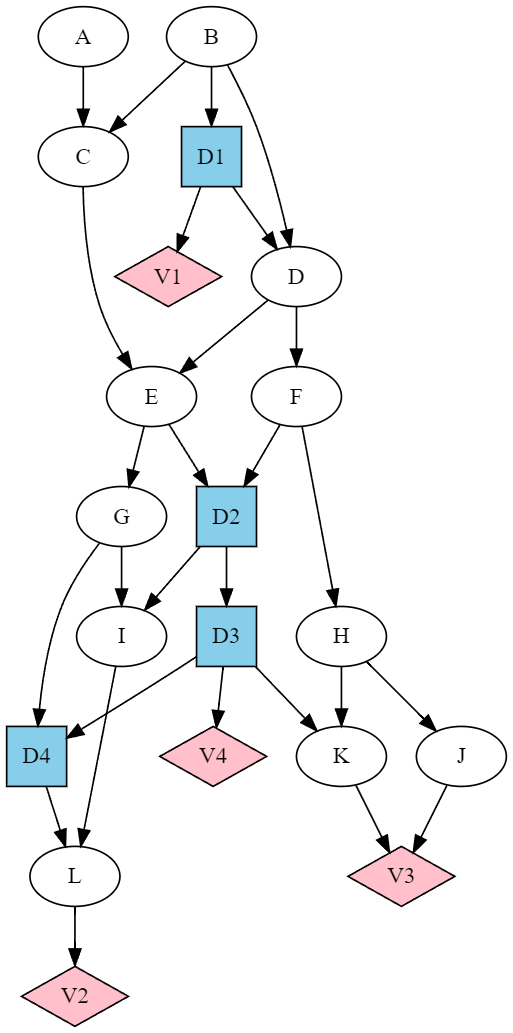
\includegraphics[width=2.3in]{influ-diag/sha-fig1.png}
%\caption{ID example from Ref.\cite{sha-influ-diag}}
%\label{fig-sha-fig1}
%\end{figure}
%
%
%\begin{figure}[h!]
%\centering
%\includegraphics[width=6in]
%{influ-diag/influ-diag-stages.jpg}
%\caption{Different decision stages for the ID shown in Fig.\ref{fig-sha-fig1}.}
%\label{fig-jensen-stages}
%\end{figure}
%
%\begin{figure}[h!]
%\centering
%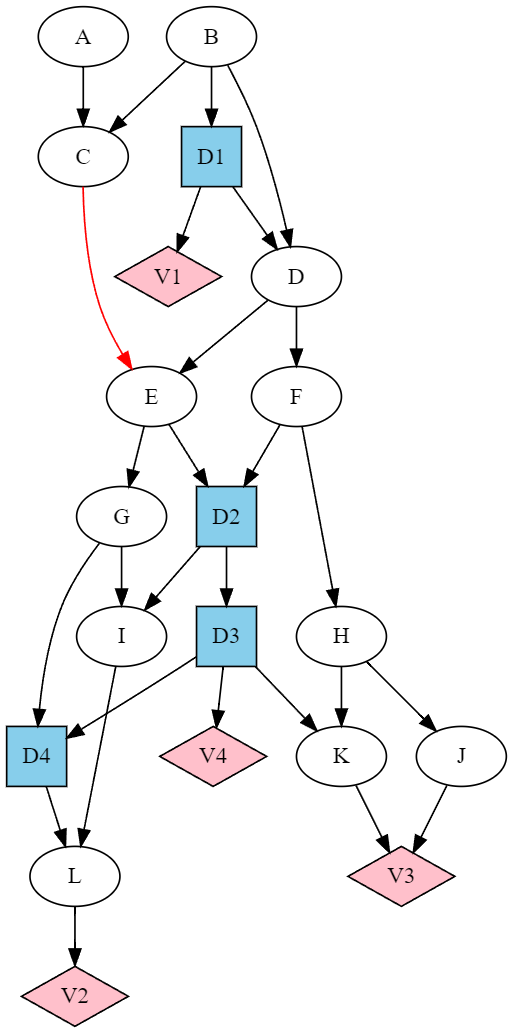
\includegraphics[width=2.3in]{influ-diag/sha-fig1a.png}
%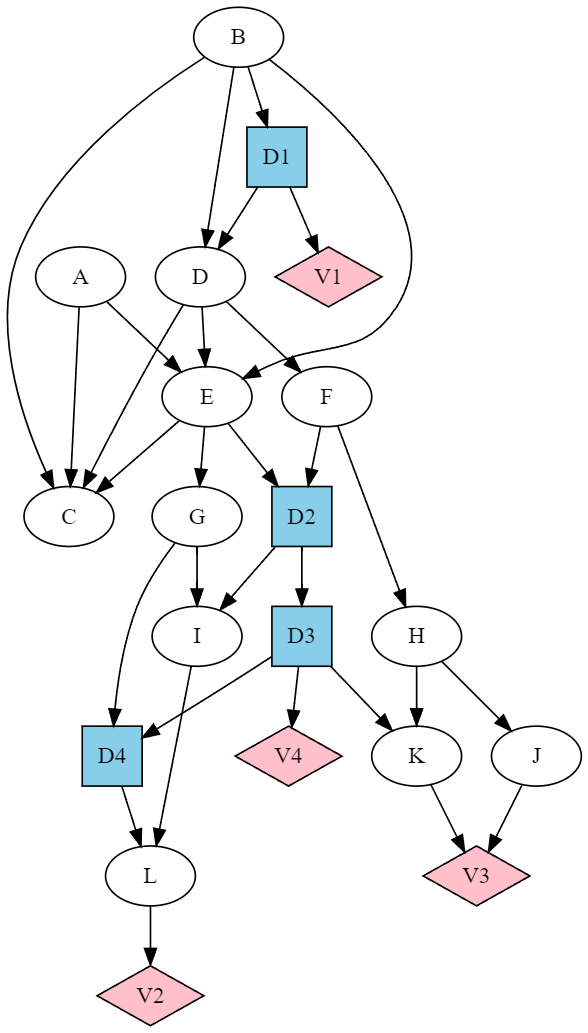
\includegraphics[width=2.3in]{influ-diag/sha-fig1b.png}
%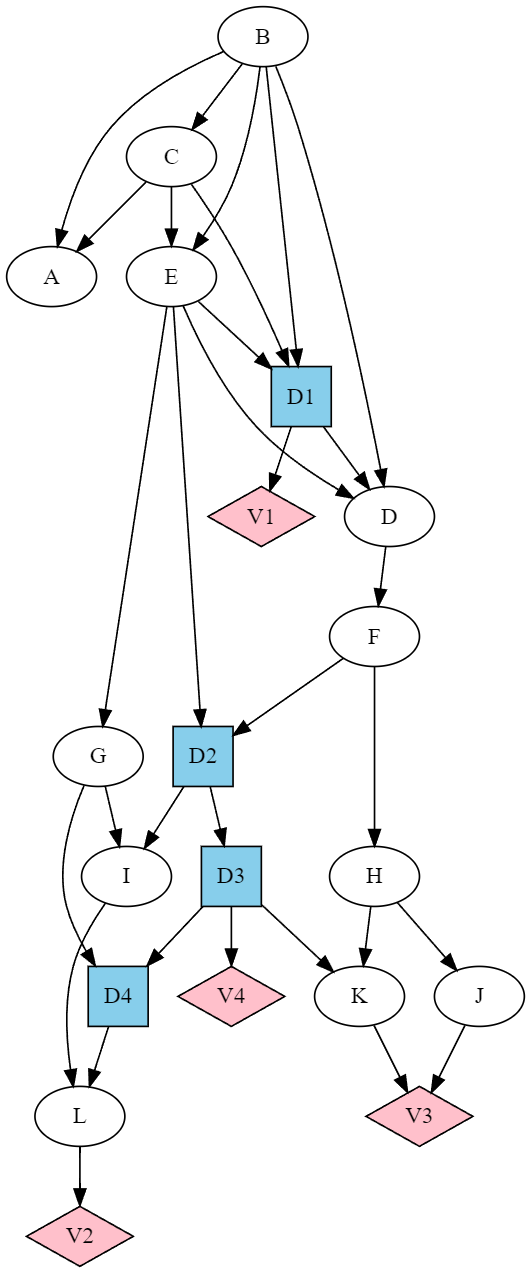
\includegraphics[width=2.3in]{influ-diag/sha-fig1c.png}
%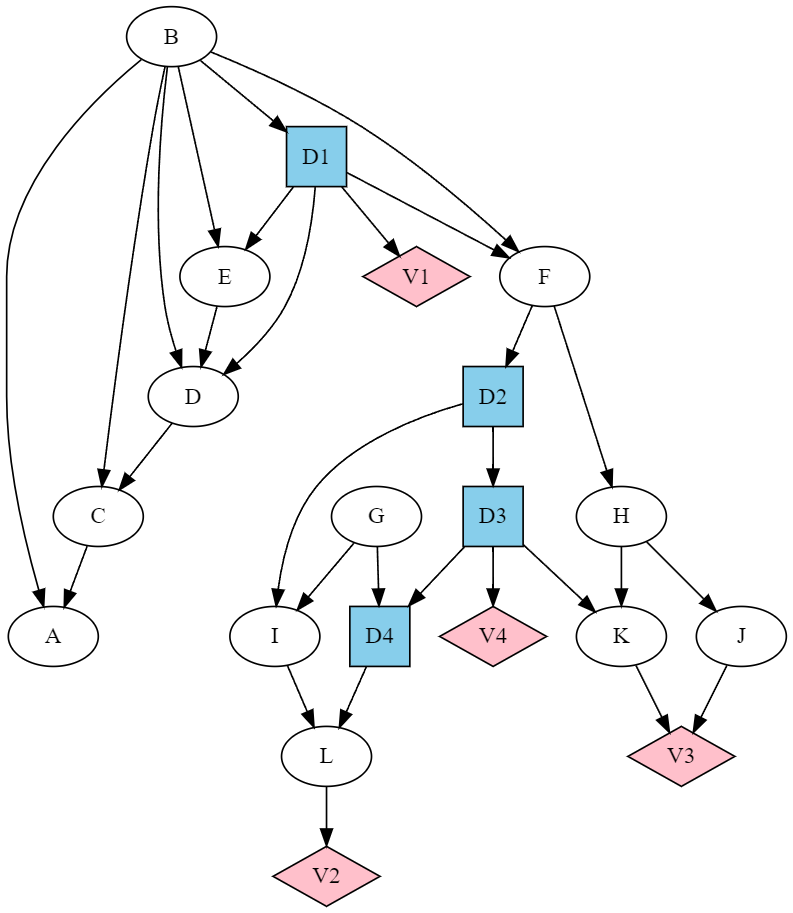
\includegraphics[width=3in]{influ-diag/sha-fig4.png}
%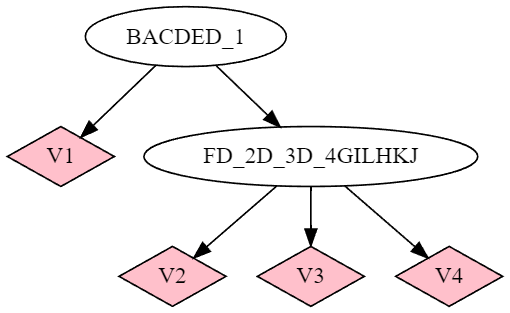
\includegraphics[width=2in]{influ-diag/sha-fig4coarse.png}
%\caption{T=Top, B=Bottom, L=Left, R=Right. {\bf TL:} the ID of Fig.\ref{fig-sha-fig1}. Arrows to be reversed in red.,
%{\bf TR:} the ID of TL after reduction to requisite
%observations. {\bf BL:} the ID of TR after reduction to a tree.
%{\bf BR:} the ID of BL after merging some nodes.}
%\label{fig-sha-fig134}
%\end{figure}
%
%

